\documentclass[12pt]{article}
\usepackage{amssymb, amsmath}
\usepackage{fancyhdr,lastpage}
\usepackage{amsmath,amsfonts,amssymb}
\usepackage{graphicx}
\usepackage{stix}
\usepackage{enumitem}
\usepackage{listings}
\tolerance 10000
\headheight 0in
\headsep 0in
\evensidemargin 0in
\oddsidemargin \evensidemargin
\textwidth 6.5in
\topmargin .25in
\textheight 8.7in

\usepackage{listings}
\usepackage{color}
 
\definecolor{codegreen}{rgb}{0,0.6,0}
\definecolor{codegray}{rgb}{0.5,0.5,0.5}
\definecolor{codepurple}{rgb}{0.58,0,0.82}
\definecolor{backcolour}{rgb}{0.95,0.95,0.92}
 

\lstdefinestyle{mystyle}{
    backgroundcolor=\color{backcolour},   
    commentstyle=\color{codegreen},
    keywordstyle=\color{magenta},
    numberstyle=\tiny\color{codegray},
    stringstyle=\color{codepurple},
    basicstyle=\footnotesize,
    breakatwhitespace=false,         
    breaklines=true,                 
    captionpos=b,                    
    keepspaces=true,                 
    numbers=left,                    
    numbersep=5pt,                  
    showspaces=false,                
    showstringspaces=false,
    showtabs=false,                  
    tabsize=2
}

\lstset{style=mystyle}


\newcommand{\CC}{{\mathbb C}}
\newcommand{\QQ}{{\mathbb Q}}
\newcommand{\RR}{{\mathbb R}}
\newcommand{\ZZ}{{\mathbb Z}}
\newcommand{\NN}{{\mathbb N}}
\newcommand{\FF}{{\mathbb F}}


\newcommand{\Zerobold}{{\boldsymbol 0}}
\newcommand{\Onebold}{{\boldsymbol 1}}
\newcommand{\xbold}{{\boldsymbol x}}

\newcommand{\mfrak}{{\mathfrak m}}

\newcommand{\Acal}{{\mathcal A}}
\newcommand{\Ncal}{{\mathcal N}}
\newcommand{\Pcal}{{\mathcal P}}
\newcommand{\Qcal}{{\mathcal Q}}

\newcommand{\sqbinom}[2]{\genfrac{[}{]}{0pt}{}{#1}{#2}}
\newcommand{\angbinom}[2]{\genfrac{\langle}{\rangle}{0pt}{}{#1}{#2}}

\newcommand{\qddx}{(d/dx)_{q}}

%\newcommand{\pfcl}{\emph{Proof of claim}}
\newenvironment{proof}{\paragraph{Proof: }}{\hfill$\blacksquare$}



\def\multiset#1#2{\ensuremath{\left(\kern-.3em\left(\genfrac{}{}{0pt}{}{#1}{#2}\right)\kern-.3em\right)}}


\DeclareMathOperator{\des}{des}
\DeclareMathOperator{\maj}{maj}
\DeclareMathOperator{\ev}{ev}
\DeclareMathOperator{\Hom}{Hom}
\DeclareMathOperator{\trace}{tr}
\DeclareMathOperator{\inv}{inv}

\newtheorem{problem}{Problem}%[section]

\begin{document}

\begin{center}
{\bf Julio Soldevilla}
\\
{\bf EECS 545 Winter 2018 --- Problem Set 5 }
\end{center}

\begin{problem}
\normalfont
Problem 1
\end{problem}

\begin{proof}
\begin{enumerate}

\item This part corresponds to the code for sigmoid function and p1.m. The code of these functions was submitted in Canvas, as the pdf said.

\item After running p1.m we got a test accuracy of 0.9540. Also, we get the following plots, the first plot ccorresponds to how the loss function behaves and the second graph corresponds to how the accuracy in the model behaves:

\begin{figure}[!htbp]
\centering
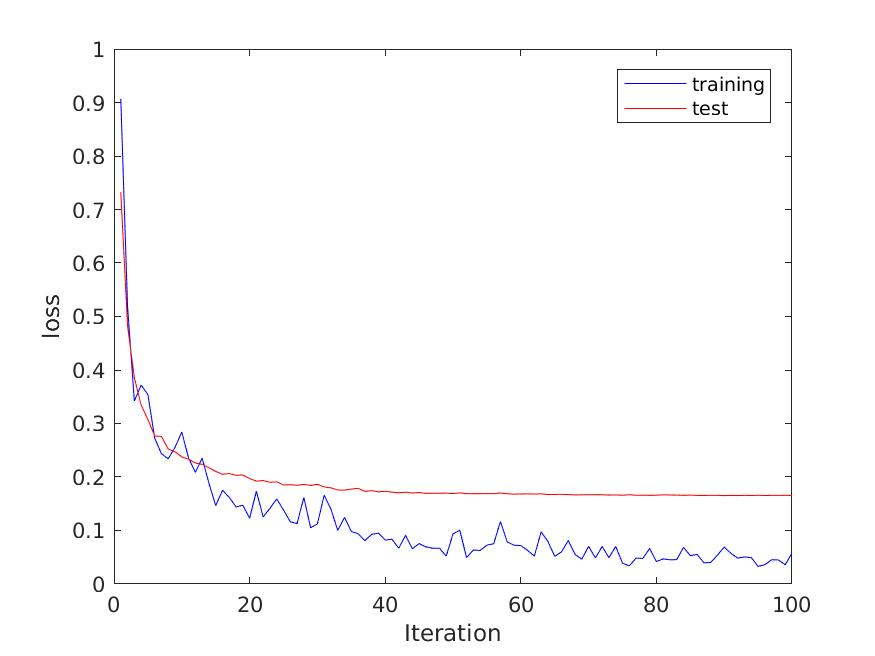
\includegraphics[width=8cm]{loss_p1.jpg}
\caption{This corresponds to the evolution of the loss function for file p1.m}
\end{figure}

\begin{figure}[!htbp]
\centering
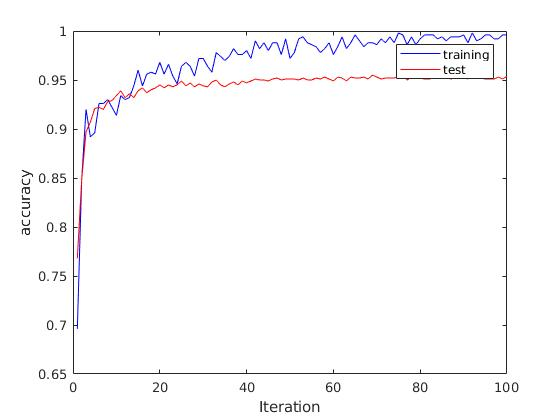
\includegraphics[width=8cm]{accuracy_p1.jpg}
\caption{This corresponds to the evolution of the accuracy in the model for file p1.m}
\end{figure}

\item To compute the learnable parameters we do the following: We know that for the first fully connected layer we have $784*50 = 39200$ weights and for the second fully connected layer we have $50*10 = 500$ weights. Also, for the first fully connected layer we have 50 bias terms and for the second fully connected layer we have $10$ bias terms. Thus, in the whole network we have $39200 + 500 + 60 = 39760$ weights that we need to learn.

\end{enumerate}
\end{proof}


\begin{problem}
\normalfont
Problem 2
\end{problem}

\begin{proof}

\begin{enumerate}
\item This part corresponds to filling out the code for p2.m. THis is presented in the Canvas file online.

\item After running p2.m, we got a test accuracy of $0.9560$. Also, we get the following plots, the first plot corresponds to how the loss function behaves in the model and the second plot corresponds to how the accuracy in the model behaves:

\begin{figure}[!htbp]
\centering
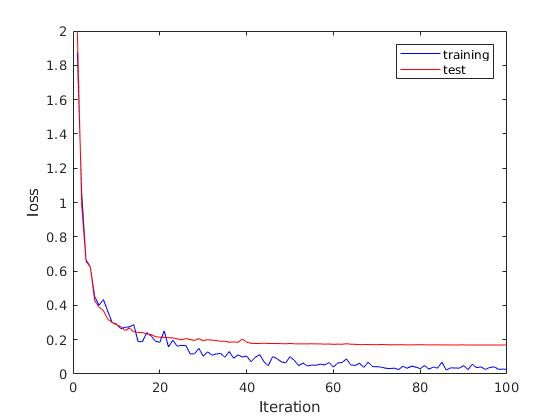
\includegraphics[width=8cm]{loss_p2.jpg}
\caption{This corresponds to the evolution of the loss function for file p2.m}
\end{figure}

\begin{figure}[!htbp]
\centering
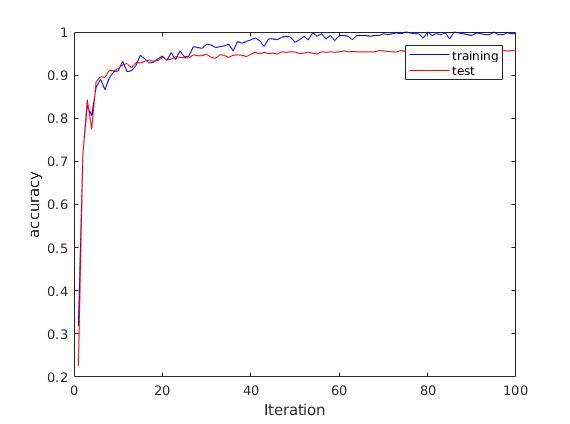
\includegraphics[width=8cm]{accuracy_p2.jpg}
\caption{This corresponds to the evolution of the accuracy in the model for file p2.m}
\end{figure}


\item For this part, we have for the first fully connected layer we have $50*784 = 39200$ weights to learn, we have $30*50 = 1500$ weights to learn for the second fully connected layer and finally we have $10*30 = 300$ weights to learn for the last fully connected layer. Also, for the first layer we have $50$ bias terms to compute, for the second layer we have $30$ bias terms to compute and finally for the last layer we have $10$ bias terms to compute. Thus, in total we have $39200 + 1500 + 300 + 90 = 41090$ parameters to learn in the model. 
\end{enumerate}

\end{proof}


\begin{problem}
\normalfont
Problem 3
\end{problem}

\begin{proof}

\begin{enumerate}

\item This part corresponds to filling out p3.m file, which is presented on Canvas.

\item For this part, after running file p3.m we get an accuracy of 0.9500. Also, we get the following plots where the first one corresponds to how the loss function behaves in the model and the second corrsponds to how the accuracy behaves in the model.

\begin{figure}[!htbp]
\centering
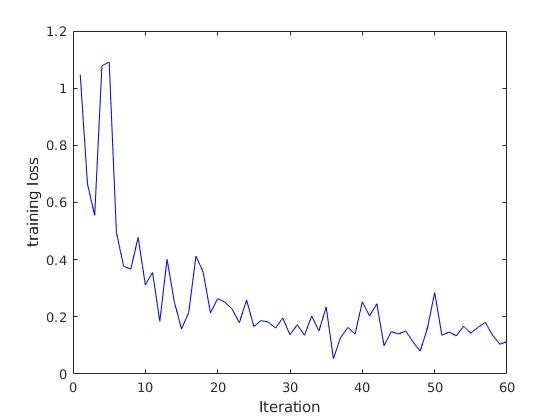
\includegraphics[width=8cm]{loss_p3.jpg}
\caption{This corresponds to the evolution of the loss function for file p3.m}
\end{figure}

\begin{figure}[!htbp]
\centering
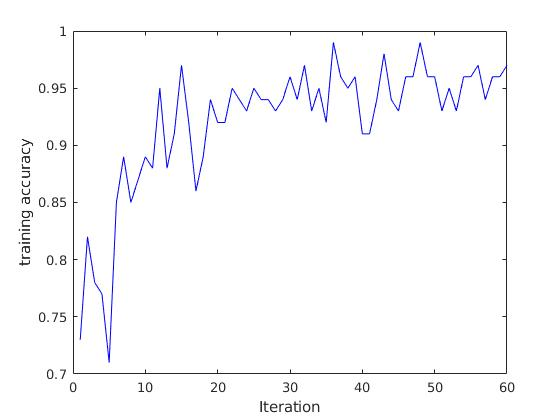
\includegraphics[width=8cm]{accuracy_p3.jpg}
\caption{This corresponds to the evolution of the accuracy in the model for file p3.m}
\end{figure}

\item For computing the learnable parameters, we first compute the parameters from the convolutional layer, where we have a filter of $9 \times 9$ from the input which has only 1 layer. We also need to consider the bias term and the fact that we will do the filtering for 15 layers of the convolution layer. Thus, for the convolution layer we will have to learn $(1 + 9 \times 9) \times 15 = 1230$ parameters, where the 1 comes from the bias term we are considering. Then for the pooling layer we don't have any new parameters to learn, since we are basically just doing a subsampling, and finally for the fully connected layer, we have to compute the weights corresponding to the $10 \times 10$ pixels on each of the layers of this final layer and for each of these pixels, we will need to connect it with 10 otuput neurons, plus consider the bias term for each of the layers in the final whole layer. Thus, we end up having $(15 \times 10 \times 10 + 1) \times 10 = (1500 + 1) * 10 = 15000 + 10$ where the 1 comes from the bias term we are condering. So in total the number of parameters we have to compute is $1230  + 15000 + 10 = 16240$

\item One of the advantages for CNN over fully connected NN is that when we are working with actual images of several pixels long, then the number of learnable parameters using CNN doesn't grow as much as when we use fully connected NN. \\

Another advantage is that CNN exploit spatial locality of the input by enforcing a local connectivity pattern between neurons of adjacent layers, whereas NN just consider the whole input, without any concern of spatial locality. Thus, CNN first creates replications of small parts of the input and then assembles them to form larger areas. NN just gets the whole image (the vectorized matrix) and tries to find relationships amongst all the pixels. This architecture of the CNN makes it faster (in general, with enought computing power) to train than NN.

\end{enumerate}

\end{proof}

\end{document}